%% Plantilla pandoc simplificada para mdpi.cls (portada: titulo, autores, simple summary, abstract)
\documentclass[water,article,submit,pdftex,moreauthors]{Definitions/mdpi}

% --- Compatibilidad con el codigo que genera pandoc/knitr ---
\providecommand{\tightlist}{\setlength{\itemsep}{0pt}\setlength{\parskip}{0pt}}
\providecommand{\pandocbounded}[1]{#1}
\makeatletter
\def\maxwidth{\ifdim\Gin@nat@width>\linewidth\linewidth\else\Gin@nat@width\fi}
\def\maxheight{\ifdim\Gin@nat@height>.9\textheight.9\textheight\else\Gin@nat@height\fi}
\makeatother
\setkeys{Gin}{width=\maxwidth,height=\maxheight,keepaspectratio}
\usepackage{booktabs}
\usepackage{longtable}
\usepackage{array}
\usepackage{multirow}
\usepackage{wrapfig}
\usepackage{float}
\usepackage{colortbl}
\usepackage{pdflscape}
\usepackage{tabularx}
\usepackage{xltabular}
\usepackage{threeparttable}
\usepackage{threeparttablex}
\usepackage[normalem]{ulem}
\usepackage{makecell}
\usepackage{xcolor}

%% Titulo y autores
\Title{Evolución del Estado de bienestar de los jóvenes europeos}
\Author{Ignacio Lacruz Mascarós, Nicolás Camacho Albiñana}

%% Simple summary y abstract

%% Referencias
\reftitle{References}
\externalbibliography{yes}

\begin{document}


\section{Introducción}\label{introducciuxf3n}

En los últimos meses, la situación de los jóvenes europeos ha vuelto al
foco público. Las protestas en España y en Francia reflejan un malestar
juvenil evidente que ha suscitado nuestro interés. En especial las
protestas relacionadas con la emancipación de los jóvenes y la situación
actual de la vivienda. En la misma localidad de Burjassot, donde
estudiamos, fue desahuciado hace unas pocas semanas un investigador de
la Universitat de València. Por esto hemos decidido conocer más sobre
este tema.

El foco de nuestra investigación será entonces el aumento de la
dificultad de independizarse de los jóvenes. Nuestra pregunta principal
será: ¿cómo ha empeorado la situación de la vivienda para los adultos
jóvenes?. Así pues, emplearemos un conjunto de datos y aplicaremos una
serie de métodos de análisis para poder responder con fundamentos y así
entender mejor cuál es la situación real en la que se encuentran los
jóvenes.

\section{Metodología: preparación del conjunto de
datos}\label{metodologuxeda-preparaciuxf3n-del-conjunto-de-datos}

\subsection{Importación de los
DataFrames}\label{importaciuxf3n-de-los-dataframes}

Los DataFrames a partir de los cuales se trabaja constan de una primera
columna donde hay información relativa al país, al sexo, a la edad y
otros parámetros que se han tenido en cuenta en la recopilación (por
ejemplo país de nacimiento, grupo social, etc.). Por tanto, el primer
paso es seleccionar solamente la información relativa al país, para lo
que usamos funciones de manipulación de strings y expresiones regulares
para seleccionar la parte de la cadena de texto que nos interesa.

Una vez hecho esto, nos damos cuenta de que las columnas corresponden a
los años de estudio, por lo que convertimos el DataFrame a formato tidy,
creando una nueva variable (columna) llamada año, en la que cada
instancia corresponde a un año distinto para cada país distinto. Las
observaciones, por tanto, se disponen en una nueva variable (columna).

Una vez cargados todos los datos que se desea estudiar, procedemos a
crear un DataFrame conjunto que los engloba. A continuación exploramos
las variables que conforman este DataFrame y determinamos cuál es la
mejor forma para llevar a cabo el análisis.

\subsection{Exploración de variables}\label{exploraciuxf3n-de-variables}

Empezaremos la exploración con una tabla que resume las características
más importantes de todas las variables del conjunto.

\begin{table}[H]
\caption{Resumen de las variables del conjunto de datos.}
\centering\footnotesize\setlength{\tabcolsep}{4pt}

\begin{tabular}{llrrrrrr}
\toprule
Variable & Type & Levels & Top level & Top count & Top frac. & Miss. freq. & Miss. frac.\\
\midrule
country & factor & 10 & DE & 27 & 0.100 & 0 & 0.000\\
year & numeric & 27 & 2000 & 10 & 0.037 & 0 & 0.000\\
age.indep & numeric & 68 & 23.7 & 13 & 0.048 & 23 & 0.086\\
earnings & numeric & 189 & 236.78 & 1 & 0.004 & 81 & 0.301\\
rel.price2015.rent & numeric & 241 & 100 & 10 & 0.037 & 10 & 0.037\\
rel.price2015.house & numeric & 177 & 95.2 & 2 & 0.007 & 89 & 0.331\\
\bottomrule
\end{tabular}
\end{table}

En esta tabla podemos notar, por ejemplo, que los valores de `Top Level'
(valor más repetido) para las variables country y year son DE
(``Deutschland'', representa Alemania, el primer país que aparece) y
2000 (el primer año que se muestrea). Esto es debido a que como todos
los países y años aparecen el mismo número de veces, la función empleada
devuelve el primero para cada caso. Pero lo verdaderamente interesante
viene analizando las dos columnas de valores perdidos (NA), Miss. freq y
Miss. frac. En estas podemos ver como en especial para las variables
relacionadas con el salario encontramos un gran porcentaje de estos
valores. Vamos a investigar más a fondo.

\pandocbounded{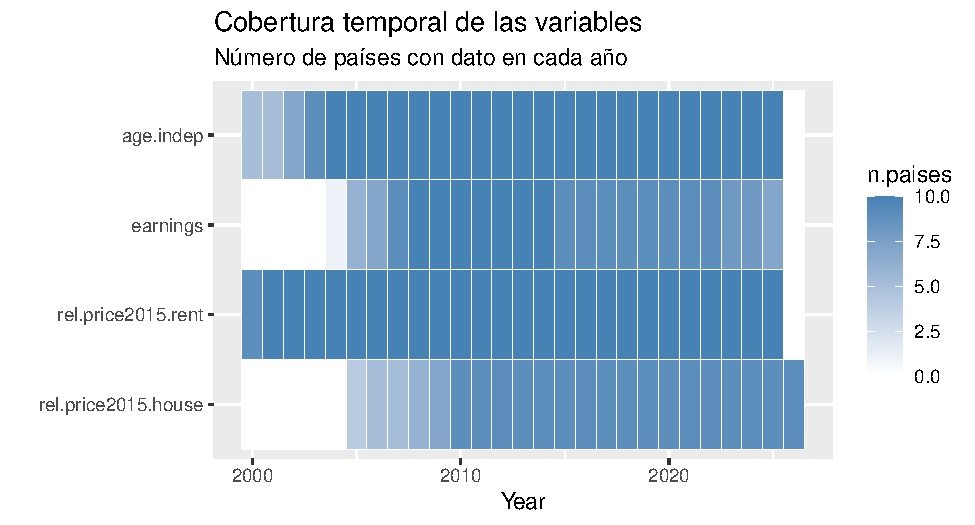
\includegraphics[keepaspectratio]{ProyectoAED_MDPI_files/figure-latex/unnamed-chunk-10-1.pdf}}

Así pues, gracias a esta gráfica podemos comprobar como en general las
variables no estan muestreadas para los 10 países más poblados hasta
2010. Esto será importante para tratar nuestro conjunto.

\subsection{Transformación de
variables}\label{transformaciuxf3n-de-variables}

Inicialmente, limitamos nuestro análisis temporal al periodo comprendido
entre 2010 y 2025, ya que antes de este año la cobertura temporal de
ciertas variables es demasiado pobre y, además, nos interesa estudiar
solamente la evolución de las variables en los años inmediatamente
anteriores, ya que remontarse demasiado en el pasado no es relevante en
este proyecto.

Como nuestro estudio se centra en la comparación de los precios de la
vivienda/alquiler con el poder adquisitivo de los jóvenes, necesitamos
establecer una escala que nos permita compararlos. De este modo,
aplicamos a las variables earnings (salarios), price.rent (precio del
alquiler) y price.house (precio de la vivienda) la siguiente
transformación:

\[ x = \frac{x}{x(t_0 = 2010)} \cdot 100 \] Esto nos permite estudiar la
evolución porcentual de las variables, ya que en el año de inicio
\(t_0 = 2010\) establecemos como referencia el \(100\%\) y, por tanto,
los valores posteriores se pueden interpretar como evoluciones en base a
un porcentaje de \(100\%\) .

Para enriquecer nuestro estudio, creamos 4 nuevas variables age.diff,
earn.diff, house.diff y rent.diff, que son la diferencia de cada valor
con su valor correspondiente al año anterior. En el caso de las 3
variables porcentuales, esto representa el aumento porcentual anual (por
ejemplo, un aumento de un \(3\%\) al año), lo cual es útil en el
posterior análisis estadístico.

\begin{verbatim}
## [1] "age.indep"   "earnings"    "price.rent"  "price.house" "age.diff"   
## [6] "earn.diff"   "house.diff"  "rent.diff"
\end{verbatim}

\section{Resultados}\label{resultados}

Con el conjunto de datos preparado, procederemos a analizarlo aplicando
distintos métodos para poder obtener conclusiones respecto a nuestra
pregunta. En este apartado se mostraran y discutiran los resultados de
dichos análisis.

\subsection{Análisis univariante: estadísticos descriptivos de las
variables
numéricas}\label{anuxe1lisis-univariante-estaduxedsticos-descriptivos-de-las-variables-numuxe9ricas}

Lo primero que uno piensa en hacer para sacar conclusiones es calcular
una serie de estadísticos básicos para todas las variables númericas
(sin contar obviamente los años). Sin embargo, para nuestro conjunto de
datos hay que tener en cuenta también un matiz importante.

Si intentáramos calcular por ejemplo la media y la desviación típica
para cada variable del conjunto de datos en formato tidy, llegaríamos a
resultados que carecen de sentido. Esto es porque estaríamos agrupando
todos los valores muestreados para cada país. Lo que se debería hacer es
calcular una media y una desviación estándar para todos los valores de
cada país de forma separada, y compararlas entre sí. En la siguiente
tabla recogemos estos resultados para los 5 países más poblados del
conjunto.

\begin{table}[H]
\caption{Media y desviación típica (SD) por país de las variables numéricas (5 países más poblados).}
\centering\footnotesize\setlength{\tabcolsep}{3pt}
\resizebox{\ifdim\width>\linewidth\linewidth\else\width\fi}{!}{%

\begin{tabular}{lrrrrrrrrrr}
\toprule
 & \multicolumn{2}{c}{DE} & \multicolumn{2}{c}{FR} & \multicolumn{2}{c}{IT} & \multicolumn{2}{c}{ES} & \multicolumn{2}{c}{PL} \\
\cmidrule(lr){2-3}\cmidrule(lr){4-5}\cmidrule(lr){6-7}\cmidrule(lr){8-9}\cmidrule(lr){10-11}
Variable & Mean & SD & Mean & SD & Mean & SD & Mean & SD & Mean & SD\\
age.indep & 23.86 & 0.14 & 23.69 & 0.19 & 30.01 & 0.16 & 29.46 & 0.67 & 27.84 & 0.60\\
earnings & 127.28 & 36.31 & 97.72 & 6.31 & 95.54 & 5.87 & 87.16 & 14.62 & 149.82 & 49.57\\
price.rent & 111.25 & 7.99 & 107.06 & 4.26 & 106.70 & 4.40 & 103.34 & 4.10 & 129.74 & 30.02\\
price.house & 142.52 & 33.32 & 114.58 & 12.41 & 90.97 & 6.38 & 92.06 & 16.35 & 122.78 & 36.26\\
age.diff & 0.00 & 0.13 & 0.02 & 0.26 & 0.03 & 0.11 & 0.12 & 0.22 & -0.09 & 0.44\\
earn.diff & 7.38 & 20.11 & 0.34 & 6.79 & -0.34 & 6.32 & 0.60 & 10.51 & 12.35 & 20.83\\
house.diff & 5.49 & 8.36 & 2.06 & 4.06 & -0.20 & 3.14 & 1.89 & 7.03 & 6.92 & 8.89\\
rent.diff & 1.71 & 0.48 & 1.10 & 0.89 & 1.22 & 1.41 & 0.87 & 1.11 & 6.06 & 5.68\\
\bottomrule
\end{tabular}}
\end{table}

En este caso es interesante notar la gran diferencia en las edades
medias de emancipación para los distintos países. En Francia y Alemania
esta es mucho menor que en España y en Italia, por ejemplo. Esto también
se alinea con las recientes manifestaciones a lo largo del país español,
todas relacionadas con la situación actual de la vivienda.

También podemos destacar unas altas desviaciones estándar en general
para los salarios y para los precios de la vivienda. Aquí hay mucha más
variabilidad incluso dentro de los mismos países.

Para completar nuestro análisis y poder contestar a nuestra hemos
decidido a continuación estudiar con más profundidad el aumento
porcentual de los salarios, el precio del alquiler y de la vivienda,
muestreado por las variables acabadas en .diff. Así, podremos comparar
las medias de cada uno de estos aumentos y así poder ver cuál es mayor.

\subsection{Media del aumento anual por país: salarios, alquiler y
vivienda}\label{media-del-aumento-anual-por-pauxeds-salarios-alquiler-y-vivienda}

Mostramos primero en la siguiente tabla las medias de los aumentos
comentados para los 10 países más poblados, así como la diferencia entre
la media del aumento de los salarios y la media de los aumentos de los
precios de la vivienda y el alquiler.

\begin{table}[H]
\caption{Media anual del aumento (\%) de los precios de la vivienda, del alquiler y de los salarios en 2010-2020, y diferencia entre salarios y precios (p.p.). Los salarios crecen más que la vivienda en 4 de 9 países y más que el alquiler en 4 de 9.}
\centering\footnotesize

\begin{tabular}{lrrrrr}
\toprule
Country & House & Rent & Earnings & Earn.$-$House & Earn.$-$Rent\\
\midrule
DE & 6.12 & 1.47 & 8.28 & 2.16 & 6.81\\
CZ & 5.65 & 2.66 & 4.36 & -1.29 & 1.70\\
BE & 2.79 & 1.44 & 0.31 & -2.48 & -1.13\\
PL & 2.59 & 3.15 & 6.69 & 4.10 & 3.53\\
NL & 2.47 & 2.99 & 0.13 & -2.35 & -2.87\\
FR & 1.78 & 0.73 & -0.09 & -1.87 & -0.83\\
RO & 0.46 & 1.76 & 13.49 & 13.04 & 11.73\\
ES & -0.53 & 0.39 & -1.13 & -0.60 & -1.52\\
IT & -1.49 & 0.65 & -0.34 & 1.15 & -0.99\\
\bottomrule
\end{tabular}
\end{table}

Fijémonos en que hay 4 países para los cuales ambas diferencias son
negativas, y que entre estos podemos encontrar a España y Francia. De
hecho, todos estos países (Países Bajos, Bélgica, España y Francia) los
podemos encontrar al oesta/la parte central de Europa, mientras que los
países que presentan ambas diferencias positivas se situan más hacia el
este.

Podemos estudiar la distribución de estos aumentos anuales en forma de
histogramas. En este caso para poder visualizarlo nos quedamos con un
subconjunto de los países: España y Francia por estar más presentes en
la actualidad y Polonia como caso diferente para poder comparar.

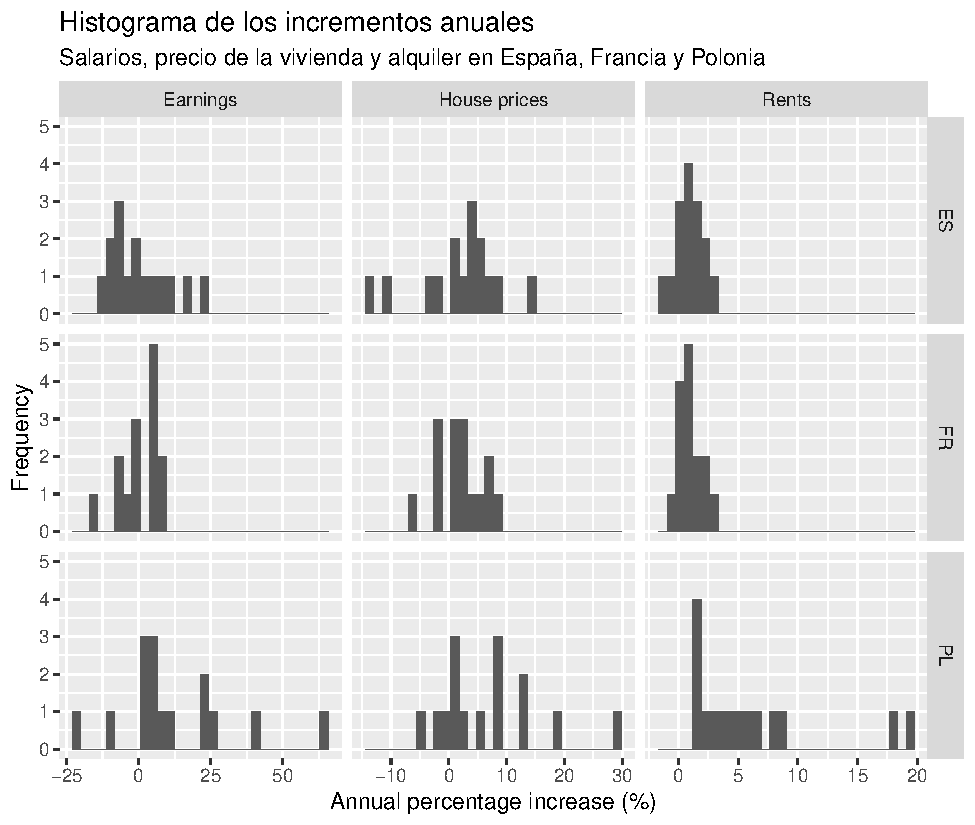
\includegraphics[width=0.8\linewidth]{ProyectoAED_MDPI_files/figure-latex/unnamed-chunk-17-1}

En general podemos identificar como las distribuciones son bastante
similares en España y Francia, pero en Polonia encontramos valores muy
separados.

Para finalizar con este análisis en la siguiente gráfica podemos
visualizar los aumentos medios para cada uno de los 10 países más
poblados, así como las diferencias previamente discutidas.

\pandocbounded{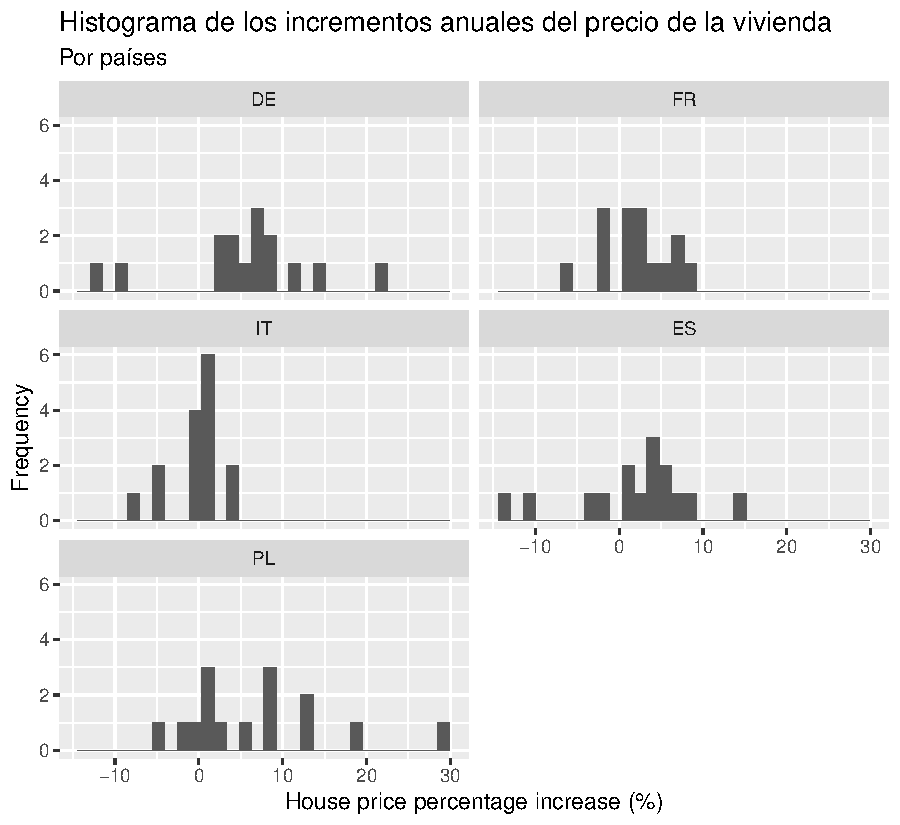
\includegraphics[keepaspectratio]{ProyectoAED_MDPI_files/figure-latex/unnamed-chunk-18-1.pdf}}

Destacan aquí los puntos referentes a Rumania, como casos aislados que
no representan fielmente la media europea. En general, podemos entender
el descontento general de los jóvenes europeos viendo como la mayoría de
estas diferencias entre salarios y precio del alquiler y la vivienda
quedan en la parte negativa.

\subsection{Edad de emancipación}\label{edad-de-emancipaciuxf3n}

A continuación se muestra la evolución temporal de la edad de
emancipación por países, así como la evolución de la media de todos
ellos:

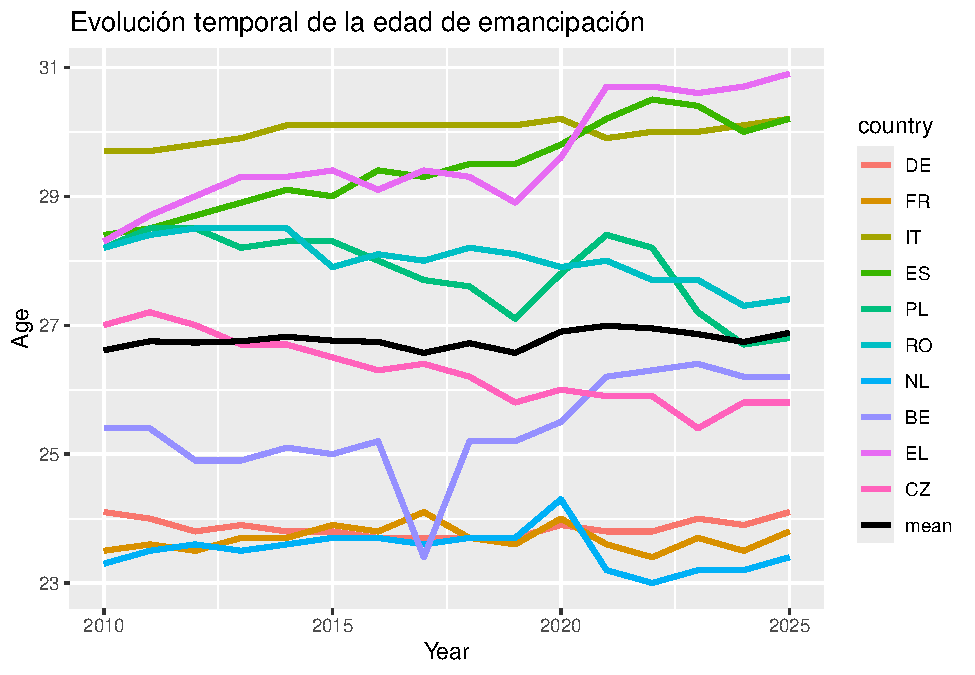
\includegraphics[width=0.8\linewidth]{ProyectoAED_MDPI_files/figure-latex/unnamed-chunk-19-1}

En la siguiente tabla observamos por países la edad de emancipación
media en estos 15 años, el aumento anual medio (en años) y la diferencia
total en la edad de emancipación en todo este tiempo.

\begin{table}[H]
\centering
\caption{\label{tab:unnamed-chunk-20}Edad de emancipación media y diferencias anuales}
\centering
\begin{tabular}[t]{lrrrr}
\toprule
country & n.years & media & media.diff & total.dif\\
\midrule
DE & 16 & 23.86 & 0.00 & 0.0\\
FR & 16 & 23.69 & 0.02 & 0.3\\
IT & 16 & 30.01 & 0.03 & 0.5\\
ES & 16 & 29.46 & 0.12 & 1.8\\
PL & 16 & 27.84 & -0.09 & -1.4\\
\addlinespace
RO & 16 & 28.02 & -0.05 & -0.8\\
NL & 16 & 23.51 & 0.01 & 0.1\\
BE & 16 & 25.41 & 0.05 & 0.8\\
EL & 16 & 29.62 & 0.17 & 2.6\\
CZ & 16 & 26.29 & -0.08 & -1.2\\
\bottomrule
\end{tabular}
\end{table}

Comprobamos que, concordantemente con la gráfica, hay diferentes
patrones de comportamiento:

\begin{enumerate}
\def\labelenumi{\arabic{enumi}.}
\item
  En España, Italia y Grecia, las edades de emancipación promedio son
  las más altas y no han hecho sino aumentar, ya que observamos
  diferencias totales positivas (de 2.6 años en Grecia por ejemplo) y
  aumentos anuales positivos (0.12 años en España al año).
\item
  En Polonia y Rumanía, las edades de emancipación comenzaron siendo
  comparables a las del grupo anterior pero han caído en los últimos
  años, ya que las diferencias totales y las medias son negativas en
  este caso.
\item
  En Países Bajos, Francia y Alemania, la situación se ha mantenido
  constante, con valores próximos a 0.
\end{enumerate}

\subsection{Análisis bivariante: estudio de la correlación entre el
aumento porcentual de los salarios y de los precios de alquiler y
vivienda}\label{anuxe1lisis-bivariante-estudio-de-la-correlaciuxf3n-entre-el-aumento-porcentual-de-los-salarios-y-de-los-precios-de-alquiler-y-vivienda}

En la siguiente gráfica se muestra la relación entre los aumentos
porcentuales anuales de los salarios y del precio de la vivienda.
Visualmente se aprecia que la tendencia es positiva:

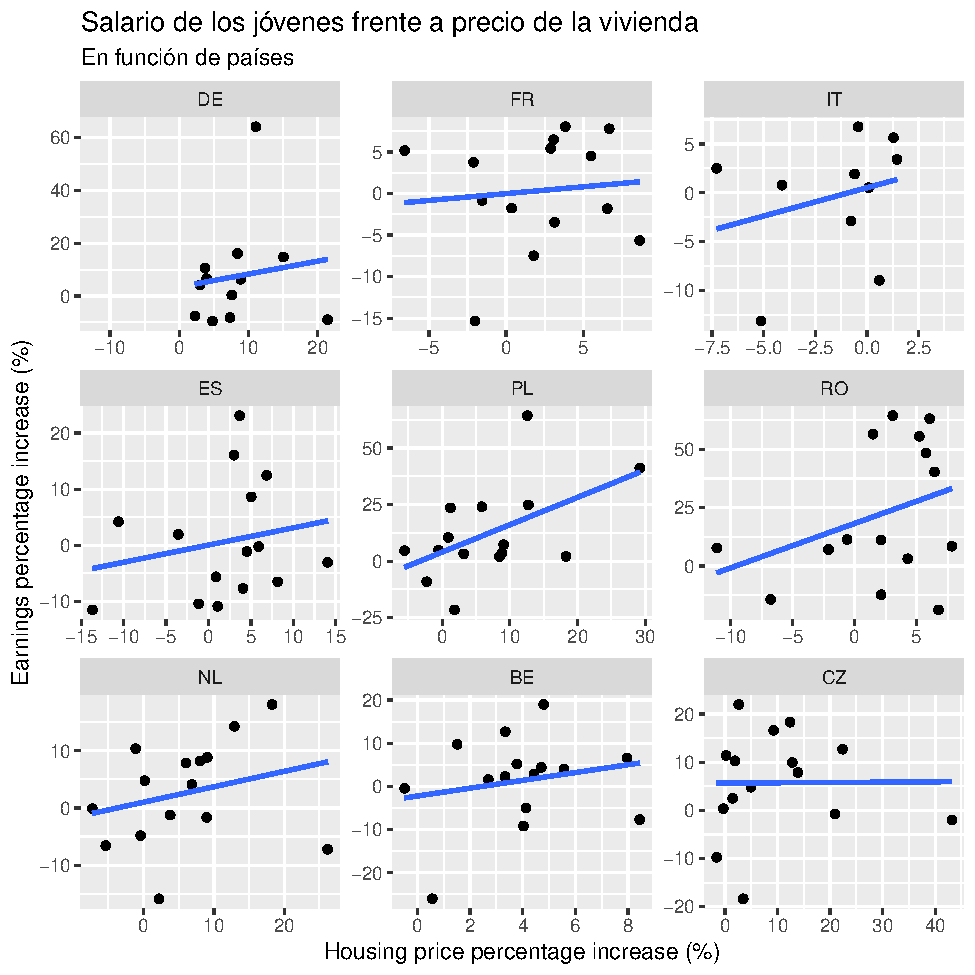
\includegraphics[width=0.8\linewidth]{ProyectoAED_MDPI_files/figure-latex/unnamed-chunk-21-1}

A continuación calculamos las correlaciones de forma numérica para cada
país, mediante los métodos de Pearson y Spearman. El caso de Polonia es
aquel con la mayor correlación, mientras que en el caso de República
Checa, es casi nula. En casi la totalidad de los casos, la correlación
es muy baja, lo que indica que la conexión intrínseca entre subidas
salariales y subidas en el precio de la vivienda es muy débil.

\begin{table}[H]
\centering
\caption{\label{tab:unnamed-chunk-22}Correlaciones entre salario y precio de la vivienda}
\centering
\begin{tabular}[t]{lrr}
\toprule
country & cor.pearson & cor.spearman\\
\midrule
DE & 0.14 & 0.22\\
FR & 0.10 & 0.13\\
IT & 0.27 & 0.35\\
ES & 0.21 & 0.23\\
PL & 0.52 & 0.39\\
\addlinespace
RO & 0.34 & 0.17\\
NL & 0.26 & 0.30\\
BE & 0.21 & 0.21\\
CZ & 0.01 & 0.10\\
\bottomrule
\end{tabular}
\end{table}

A continuación, calculamos el valor numérico de la pendiente de la
regresión lineal mostrada en la figura: salvo en el caso de Rumanía y
Polonia, donde los aumentos en el salario son en promedio superiores a
los de la vivienda (pendiente mayor a 1), en los demás casos tenemos la
situación contraria, lo que muestra que la variabilidad del precio de la
vivienda es mayor que la de los salarios.

\begin{table}[H]
\centering
\caption{\label{tab:unnamed-chunk-23}Pendientes de salario frente a precio de la vivienda}
\centering
\begin{tabular}[t]{lr}
\toprule
country & slope\\
\midrule
DE & 0.49\\
FR & 0.16\\
IT & 0.58\\
ES & 0.31\\
PL & 1.21\\
\addlinespace
RO & 1.91\\
NL & 0.27\\
BE & 0.90\\
CZ & 0.01\\
\bottomrule
\end{tabular}
\end{table}

Ahora repetimos el mismo análisis bivariante con los aumentos salariales
frente a los aumentos del alquiler. Vemos que las tendencias son en
general positivas, como en el caso de la vivienda, salvo para Italia,
donde salarios y alquileres están ligeramente correlacionados de manera
negativa.

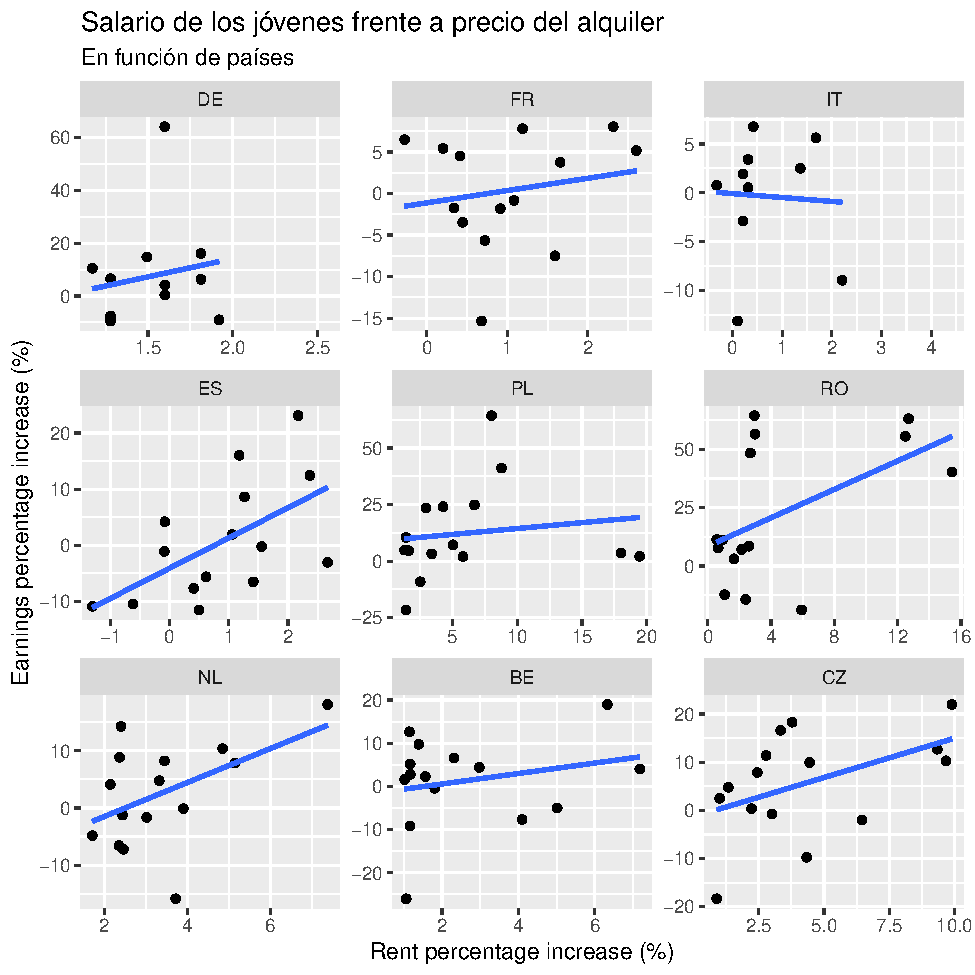
\includegraphics[width=0.8\linewidth]{ProyectoAED_MDPI_files/figure-latex/unnamed-chunk-24-1}

Las correlaciones ahora son algo mayores que en el caso anterior, pero
aun así no son significativas, por lo que no podemos deducir una
relación intrínseca entre ambos aumentos.

\begin{table}[H]
\centering
\caption{\label{tab:unnamed-chunk-25}Correlaciones entre salario y alquiler}
\centering
\begin{tabular}[t]{lrr}
\toprule
country & cor.pearson & cor.spearman\\
\midrule
DE & 0.17 & 0.15\\
FR & 0.18 & 0.09\\
IT & -0.05 & 0.35\\
ES & 0.57 & 0.55\\
PL & 0.14 & 0.24\\
\addlinespace
RO & 0.51 & 0.44\\
NL & 0.48 & 0.35\\
BE & 0.24 & 0.21\\
CZ & 0.47 & 0.48\\
\bottomrule
\end{tabular}
\end{table}

En el estudio de las pendientes, como ya se ha comentado, hay valores
positivos en la mayoría de casos y además son mayores que en el caso de
la vivienda, luego la variabilidad de los salarios es mayor que la del
alquiler (salvo en Italia y Polonia).

\begin{table}[H]
\centering
\caption{\label{tab:unnamed-chunk-26}Pendientes de salario frente a alquiler}
\centering
\begin{tabular}[t]{lr}
\toprule
country & slope\\
\midrule
DE & 13.85\\
FR & 1.48\\
IT & -0.40\\
ES & 5.40\\
PL & 0.52\\
\addlinespace
RO & 3.05\\
NL & 2.97\\
BE & 1.21\\
CZ & 1.63\\
\bottomrule
\end{tabular}
\end{table}

En las siguientes gráficas se muestra, de forma superpuesta y para cada
país, la evolución temporal de los salarios, el precio de la vivienda y
los alquileres. Visualmente apreciamos diferentes casuísticas:

\begin{enumerate}
\def\labelenumi{\arabic{enumi}.}
\item
  En Polonia y Rumanía, los salarios han aumentado por encima de los
  precios de la vivienda y del alquiler.
\item
  En Italia, los salarios han aumentado por encima del precio de la
  vivienda pero no del alquiler.
\item
  En República Checa, los salarios han aumentado por encima del alquiler
  pero no de la vivienda.
\item
  En el resto de países, los salarios están por debajo de ambos precios.
\end{enumerate}

\pandocbounded{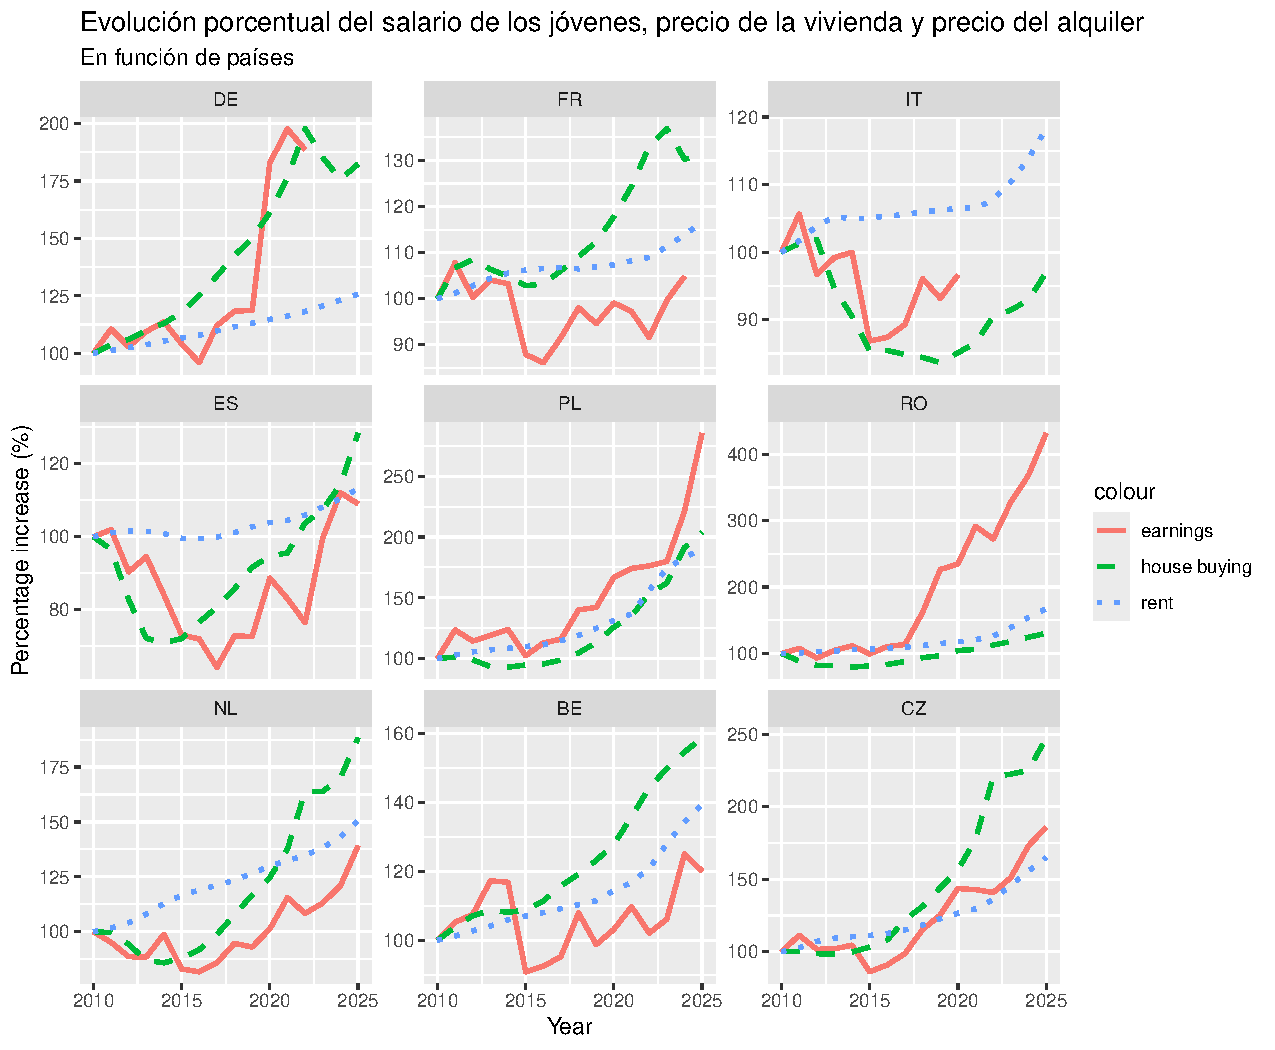
\includegraphics[keepaspectratio]{ProyectoAED_MDPI_files/figure-latex/unnamed-chunk-27-1.pdf}}

En la siguiente tabla vemos los aumentos totales de los 3 índices
durante los últimos 15 años, así como las diferencias entre ellos
(earn.m.house, earn.m.rent). Los resultados numéricos son coherentes con
los gráficos: salvo en Polonia y Rumanía, en los demás países al menos 1
de las diferencias es negativa, lo que indica que el poder adquisitivo
ha caído con respecto al precio de la vivienda, del alquiler o de ambos.

\begin{table}[H]
\centering
\caption{\label{tab:unnamed-chunk-28}Diferencias totales y evolución del poder adquisitivo}
\centering
\begin{tabular}[t]{lrrrrr}
\toprule
country & earn.total.dif & house.total.dif & rent.total.dif & earn.m.house & earn.m.rent\\
\midrule
DE & 88.59 & 97.71 & 18.12 & -9.12 & 70.47\\
FR & 4.79 & 30.31 & 13.88 & -25.52 & -9.09\\
IT & -3.41 & -14.90 & 6.51 & 11.49 & -9.92\\
ES & 8.97 & 28.28 & 13.10 & -19.31 & -4.13\\
PL & 185.25 & 103.82 & 90.88 & 81.43 & 94.37\\
\addlinespace
RO & 331.60 & 30.52 & 67.14 & 301.08 & 264.46\\
NL & 39.04 & 88.30 & 50.65 & -49.26 & -11.61\\
BE & 20.06 & 58.78 & 39.38 & -38.73 & -19.32\\
CZ & 85.80 & 147.48 & 64.96 & -61.68 & 20.84\\
\bottomrule
\end{tabular}
\end{table}

\section{Conclusiones}\label{conclusiones}

Inicialmente, a partir de la evolución de la edad de emancipación
podemos concluir que países como España, Italia, Grecia y Bélgica han
empeorado su situación, mientras que Polonia, Rumanía y República Checa
la han mejorado. Francia, Alemania y Países Bajos, por su parte, se
mantienen en un escenario similar. Por tanto, vemos que en general, los
países occidentales (salvo Alemania y Francia) viven una peor situación,
mientras que los orientales la han mejorado.

A partir de los incrementos anuales, concluimos que, cada año de media,
los ciudadanos españoles e italianos ven mermado su poder adquisitivo
respecto al aquiler, los franceses y checos respecto a la vivienda y los
neerlandeses y belgas respecto a ambos. Se aprecia de nuevo el buen
desempeño de alemanes, rumanos y polacos, por lo que la situación de los
países orientales resulta ser mejor que la de los occidentales en este
aspecto también.

El análisis bivariante empeora todavía más el diagnóstico, ya que nos
muestra que los aumentos anuales salariales no solo se han quedado
rezagados con respecto a la vivienda/alquiler, sino que además sus
evoluciones no están correlacionadas, es decir, el aumento de precio de
la vivienda no implica necesariamente un aumento salarial para la gente
joven. Esto puede deberse al hecho de que los propietarios de vivienda
son por lo general gente de mediana y avanzada edad, por lo que un
aumento del precio de los alquileres le es económicamente rentable a
este grupo de edad, mientras que reduce el poder adquisitivo de la
juventud.

El caso particular de Polonia destaca de nuevo por ser aquel en el que
más correlación existe entre estas variables, al igual que en el caso de
Rumanía principalmente en los alquileres. Destacamos, por el contrario,
la situación de los alquileres italianos, que además de estar poco
correlacionados con los salarios, lo hacen de forma ligeramente
negativa, lo cual debería ser un síntoma de alarma.

Finalmente, en el análisis de las diferencias totales en salarios,
alquileres y viviendas, vemos que por lo general los sueldos han
aumentado en estos 15 años, pero los precios se han incrementado con más
fuerza, lo que provoca un balance final negativo en el caso de Francia,
España, Países Bajos y Bélgica con respecto tanto al alquiler como a la
vivienda.

En el caso de Alemania y República Checa, el balance es negativo
exclusivamente en relación a la vivienda, no al alquiler, mientras que
la situación de Italia es la opuesta, destacando en este último país que
es el único en que el salario se ha reducido de forma absoluta, lo que
lo convierte en el caso más preocupante.

Todos estos países son los que podemos englobar como occidentales,
precisamente aquellos donde se ha hecho oír el descontento social en
forma de manifestaciones y altercados, mientras que en el caso de los
orientales, como Polonia y Rumanía, vemos que la situación es la
contraria y, por tanto, esto es coherente con la ausencia de protestas
públicas en estos países.

\bibliography{mybibfile.bib}



\end{document}
